\section{Upgrading EML} \label{sec:upgrading-eml}

Morpho displays older EML packages (e.g., 2.0 or Beta 6), but will
automatically convert them to EML 2.0 for display. If a package does not
use the latest EML format, Morpho will prompt users to upgrade the EML
to the latest version (\autoref{fig:upgrade-eml-dialog}). After
completing the upgrade, you must save the data package to preserve the
changes, at which time the revision number of the document will be
incremented. Please note that if you choose not to upgrade the EML,
Morpho will not allow you to edit the document.

\begin{figure}
  \centering
    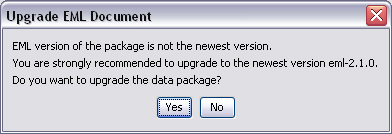
\includegraphics[width=0.7\textwidth]{images/upgrade-eml-dialog.jpg}
  \caption{Morpho prompts users to upgrade EML for older packages.}
  \label{fig:upgrade-eml-dialog}
\end{figure}

If a user chooses to upgrade the EML and the upgraded EML document is
invalid (e.g., it contains only whitespace for a required metadata
field), Morpho will prompt you to use the Correction Wizard to fix the
problem (\autoref{fig:upgrade-eml-warning}).

\begin{figure}
  \centering
    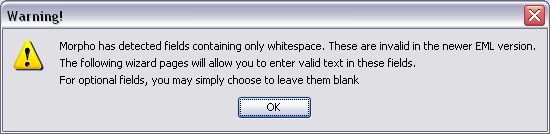
\includegraphics[width=0.7\textwidth]{images/upgrade-eml-warning.jpg}
  \caption{If Morpho detects that the upgraded EML has fields containing
    only whitespace, it will prompt you to use the correction wizard to
    specify a new value.}
  \label{fig:upgrade-eml-warning}
\end{figure}

The correction wizard (\autoref{fig:upgrade-eml-wizard}) steps you
through the blank metadata screens. Note that in some cases, you will be
required to use the Morpho Editor to supply information. The wizard will
notify you if this is the case, and will open the Morpho Editor with a
text-field to collect the missing information
(\autoref{fig:upgrade-eml-correction}). Enter the appropriate value and
click OK.

\begin{figure}
  \centering
    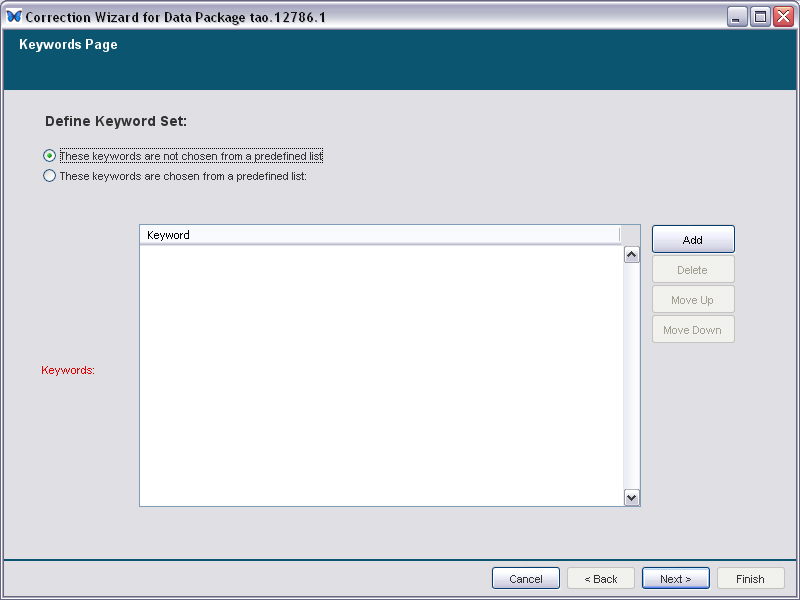
\includegraphics[width=0.7\textwidth]{images/upgrade-eml-wizard.jpg}
  \caption{Morpho's Correction Wizard prompts you to enter the required
    information.}
  \label{fig:upgrade-eml-wizard}
\end{figure}

\begin{figure}
  \centering
    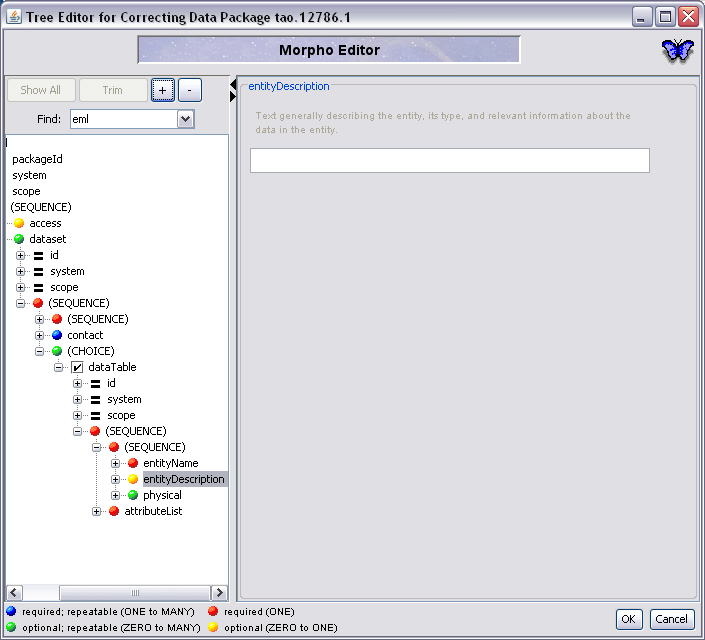
\includegraphics[width=0.7\textwidth]{images/upgrade-eml-correction.jpg}
  \caption{If required, the Correction Wizard opens the Morpho Editor to
    collect additional required information.}
  \label{fig:upgrade-eml-correction}
\end{figure}

